
    \begin{frame}{\ft{Initial Application Window}}

        \begin{annotatedFigure}{0pt}{0pt}
            {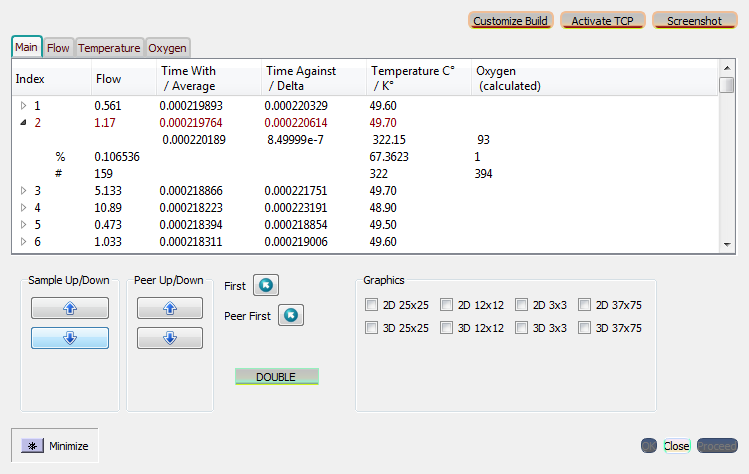
\includegraphics[scale=1]{texs/expand.png}}
            
  \node [text width=7.3cm,align=justify,fill=logoCyan!20, draw=logoBlue, 
  draw opacity=0.5,line width=1mm, fill opacity=0.9]
   at (0.74,0.465){\textbf{Using a ``tree widget" (a two-layer spreadsheet), 
  instead of a conventional spreadsheet, allows the Dataset Application to 
  distinguish primary values (those measured directly by physical devices 
  and experimental equipment) from intermediate values calculated via algorithms.}};
              
            \annotatedFigureBox{0.01,0.6}{0.75,0.77}{1}{0.75,0.6}
            
  \node [text width=7.8cm,align=justify,fill=logoCyan!20, draw=logoBlue, 
  draw opacity=0.5,line width=1mm, fill opacity=0.9]
   at (0.23,0.475){\textbf{In addition, nested rows can 
   display supplemental infomation, such as data values' 
   rank (\circled{3}) and percentage (\circled{2}) 
   (on the scale of the least to greatest 
   value) relative to all other values for each statistical parameter.}};
              
            \annotatedFigureBox{0.015,0.65}{0.1,0.69}{2}{0.1,0.69}
            \annotatedFigureBox{0.015,0.62}{0.1,0.648}{3}{0.1,0.625}                        
            
            
            
            %bl
      %      \annotatedFigureBox{0.222,0.284}{0.3743,0.4934}{B}{0.3743,0.4934}%tr
      %      \annotatedFigureBox{0.555,0.784}{0.6815,0.874}{C}{0.555,0.784}%bl
      %      \annotatedFigureBox{0.557,0.322}{0.8985,0.5269}{D}{0.8985,0.5269}%tr
  

        \end{annotatedFigure}

   %     \caption{Expanded Sample (A)}
    %    \label{fig:teaser}

    \end{frame}


